\chapter{Présentation du dashboard}
\label{ch:dashboard}
\section{Pages}
Le front-end WiFace propose les pages et les fonctionnalités suivantes:
\subsection{Login et register}

La page de login (fig \ref{fig:dashboard_login}) permet de se connecter en tant qu'administrateur au dashboard.
Au vu de la sensibilité des données, seuls les utilisateurs avec le rôle administrateur peuvent se connecter.
Une bonne pratique serait de ne pas donner ce rôle aux comptes associés aux clients Raspberry Pi.

La page register (fig \ref{fig:dashboard_register}) permet de créer un nouveau compte pour un client potentiel.
Pour créer un compte, il faut renseigner les informations suivantes:
\begin{itemize}
    \item e-mail
    \item mot de passe
    \item localisation du client
    \item rôle du client (admin ou non) 
\end{itemize}

Il est à noter que certains de ces champs sont soumis à des contraintes d'unicité ou de longueur par exemple.
Si le client doit être installé dans un nouveau lieu, il est possible de créer ce lieu sur cette page. 
Pour cela, il faut d'abord séléctionner "New Place" dans la liste déroulante. Ensuite, ajouter le lieu en cliquant sur la carte. Pour
finir, un nom doit lui être donné. 

\clearpage
\newpage
\thispagestyle{empty}
\begin{landscape}
    \centering
\thispagestyle{empty}
\begin{figure}[H]
	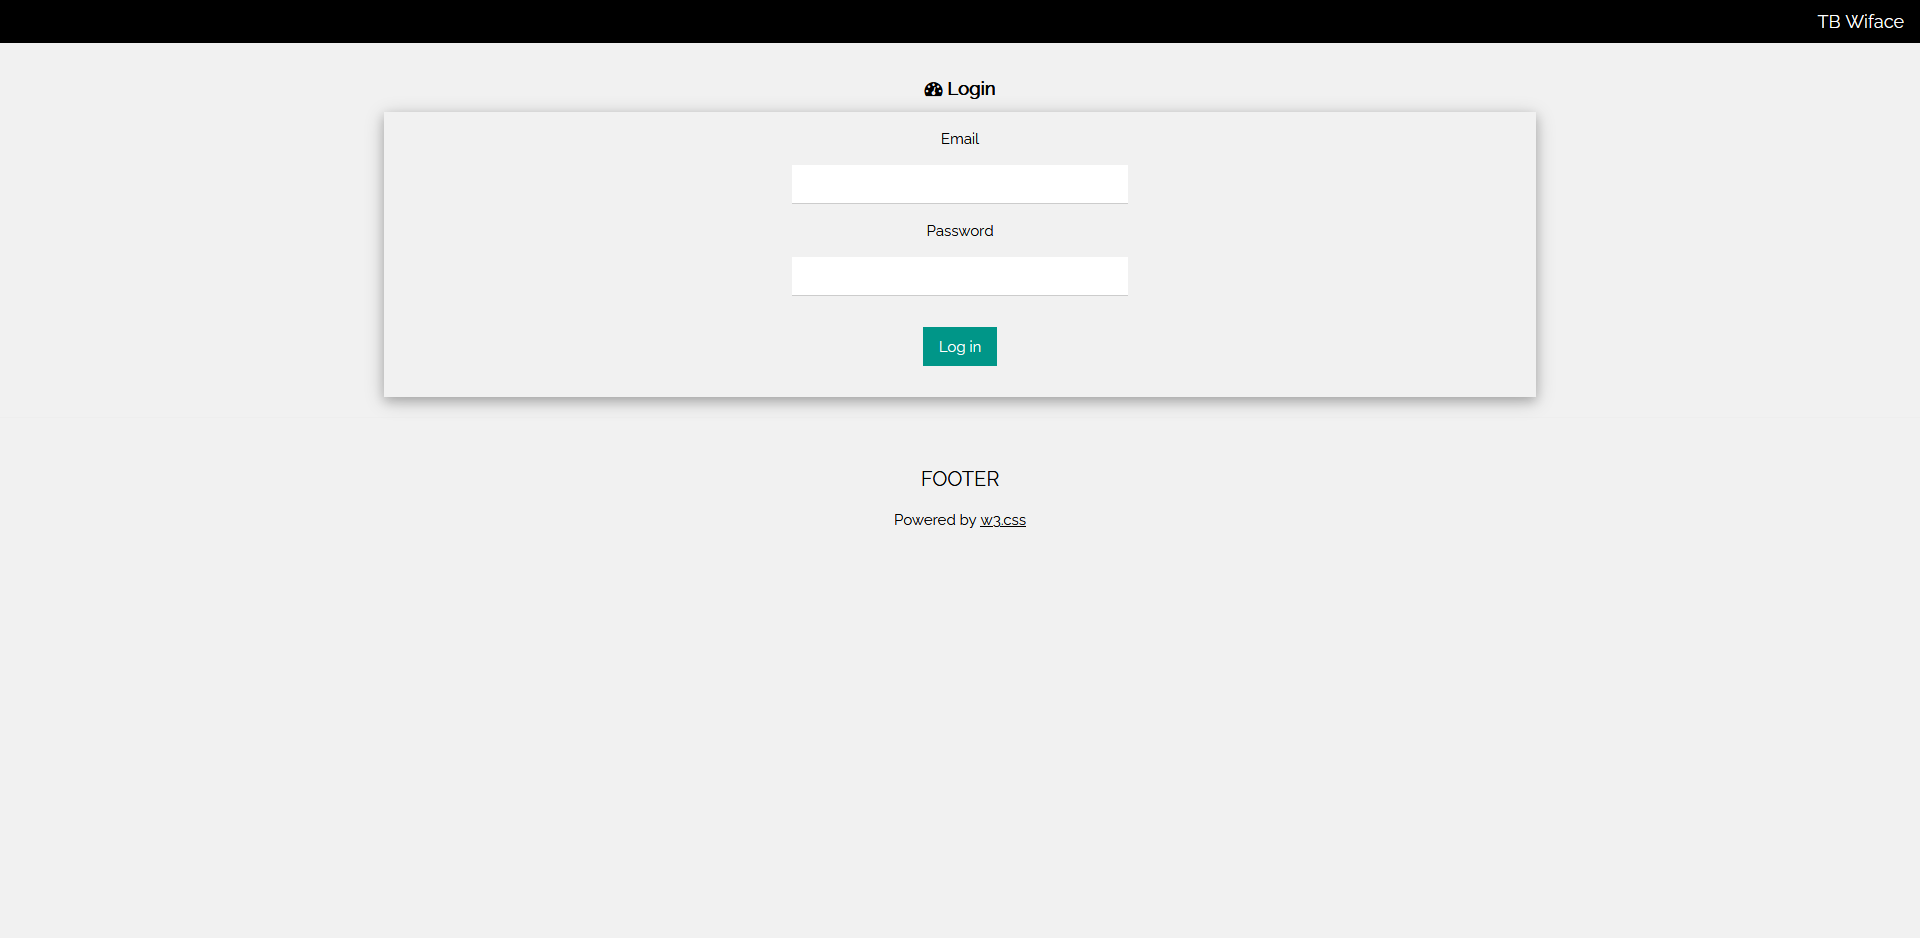
\includegraphics[width=0.95\linewidth]{images/dashboard/login.png}
	\caption{Page de login}
	\label{fig:dashboard_login}
\end{figure}
\end{landscape}

\clearpage
\newpage
\thispagestyle{empty}
\begin{landscape}
    \centering
\thispagestyle{empty}
\begin{figure}[H]
	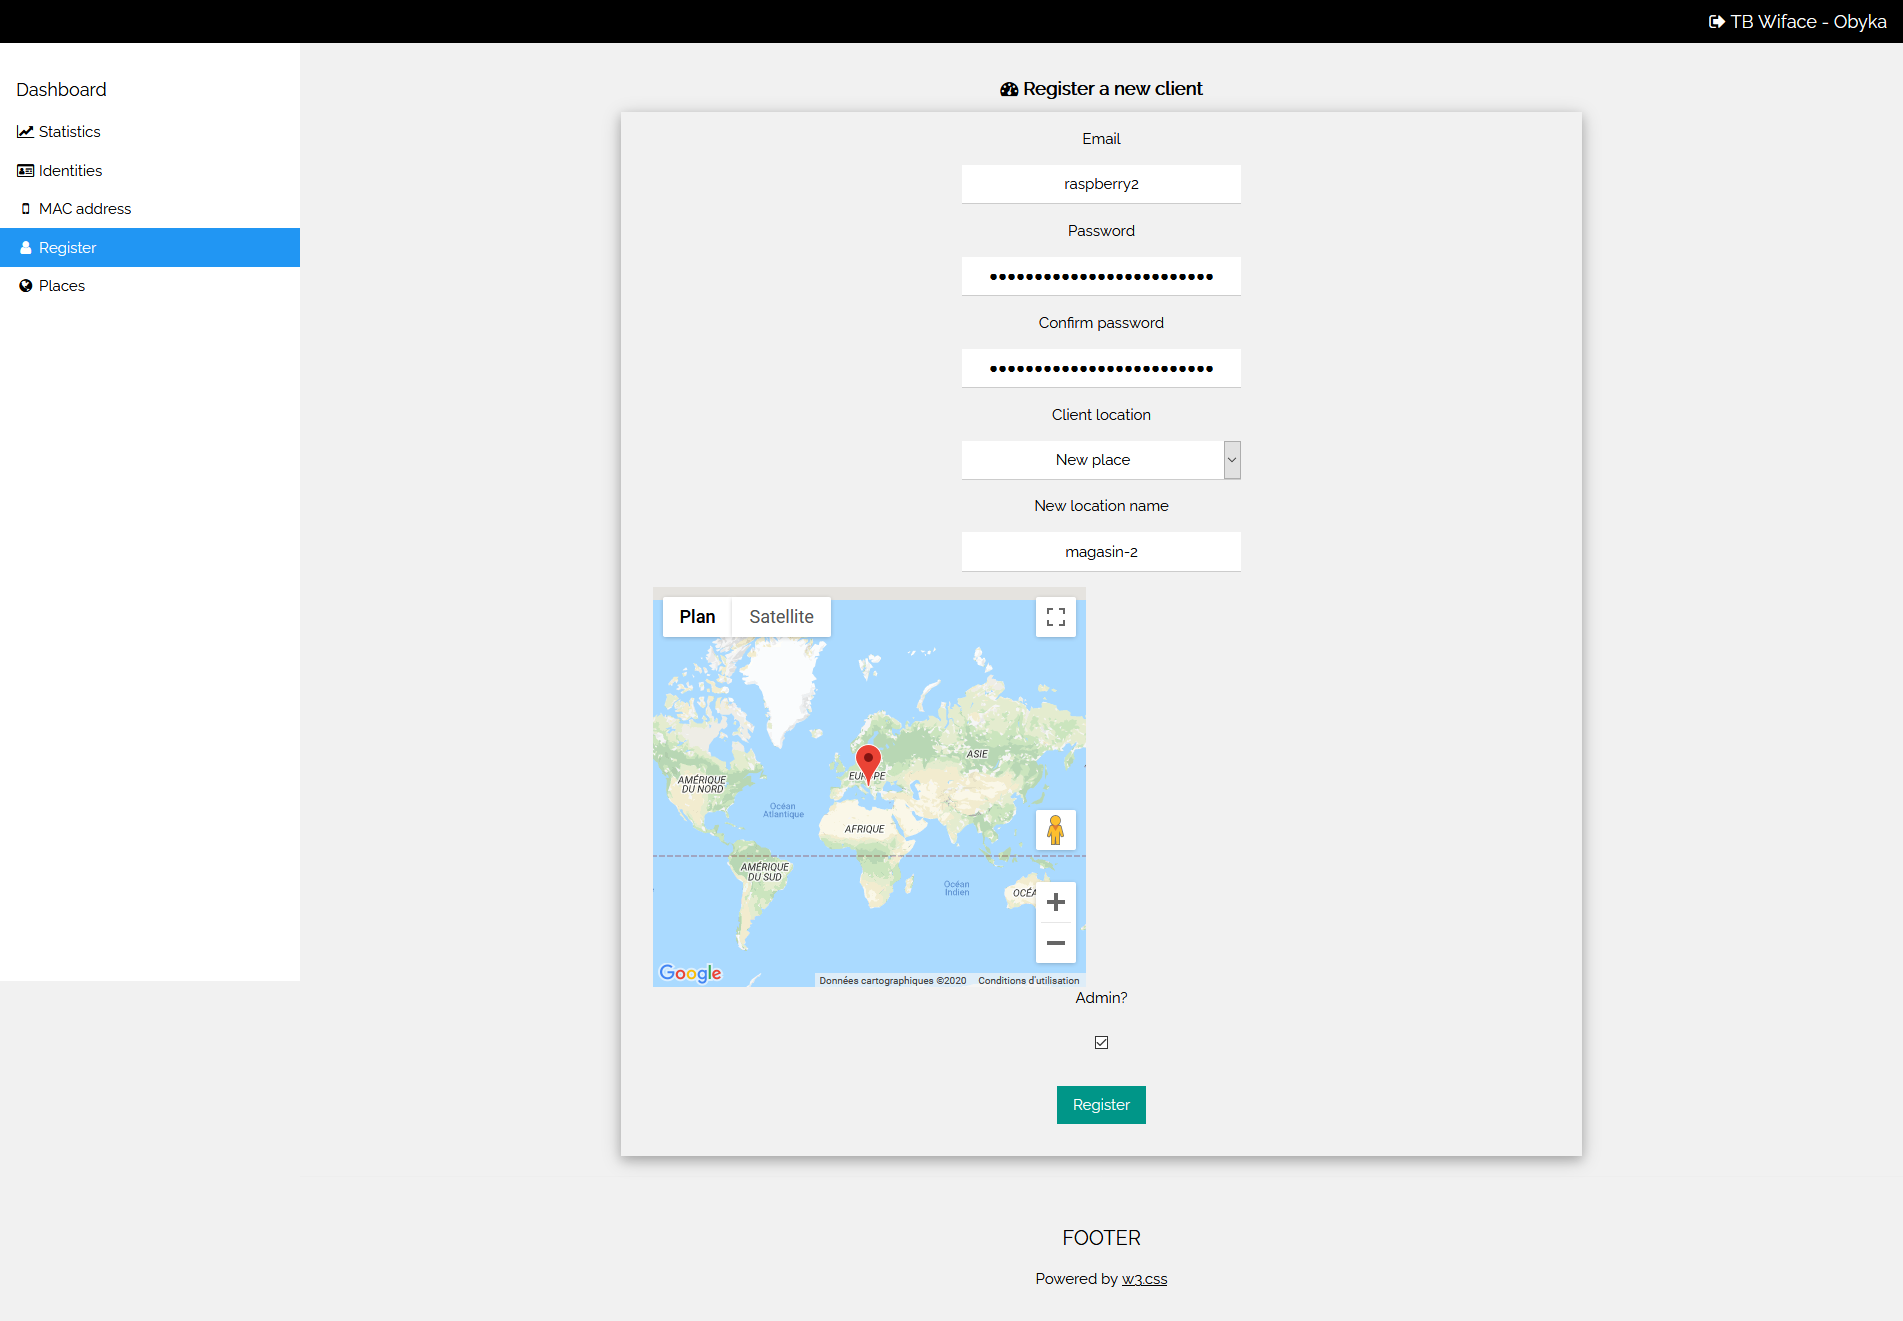
\includegraphics[width=0.95\linewidth]{images/dashboard/register.png}
	\caption{Page d'inscription}
	\label{fig:dashboard_register}
\end{figure}
\end{landscape}

\subsection{Statistiques}

La page d'accueil (fig \ref{fig:dashboard_stats}) montre quelques statistiques sur l'état de l'API WiFace (e.g Feed des derniers événements, nombre d'identités dans la base de données, etc)
et permet ainsi à un opérateur d'avoir une vue d'ensemble.
\clearpage
\newpage
\thispagestyle{empty}
\begin{landscape}
    \centering
\thispagestyle{empty}
\begin{figure}[H]
	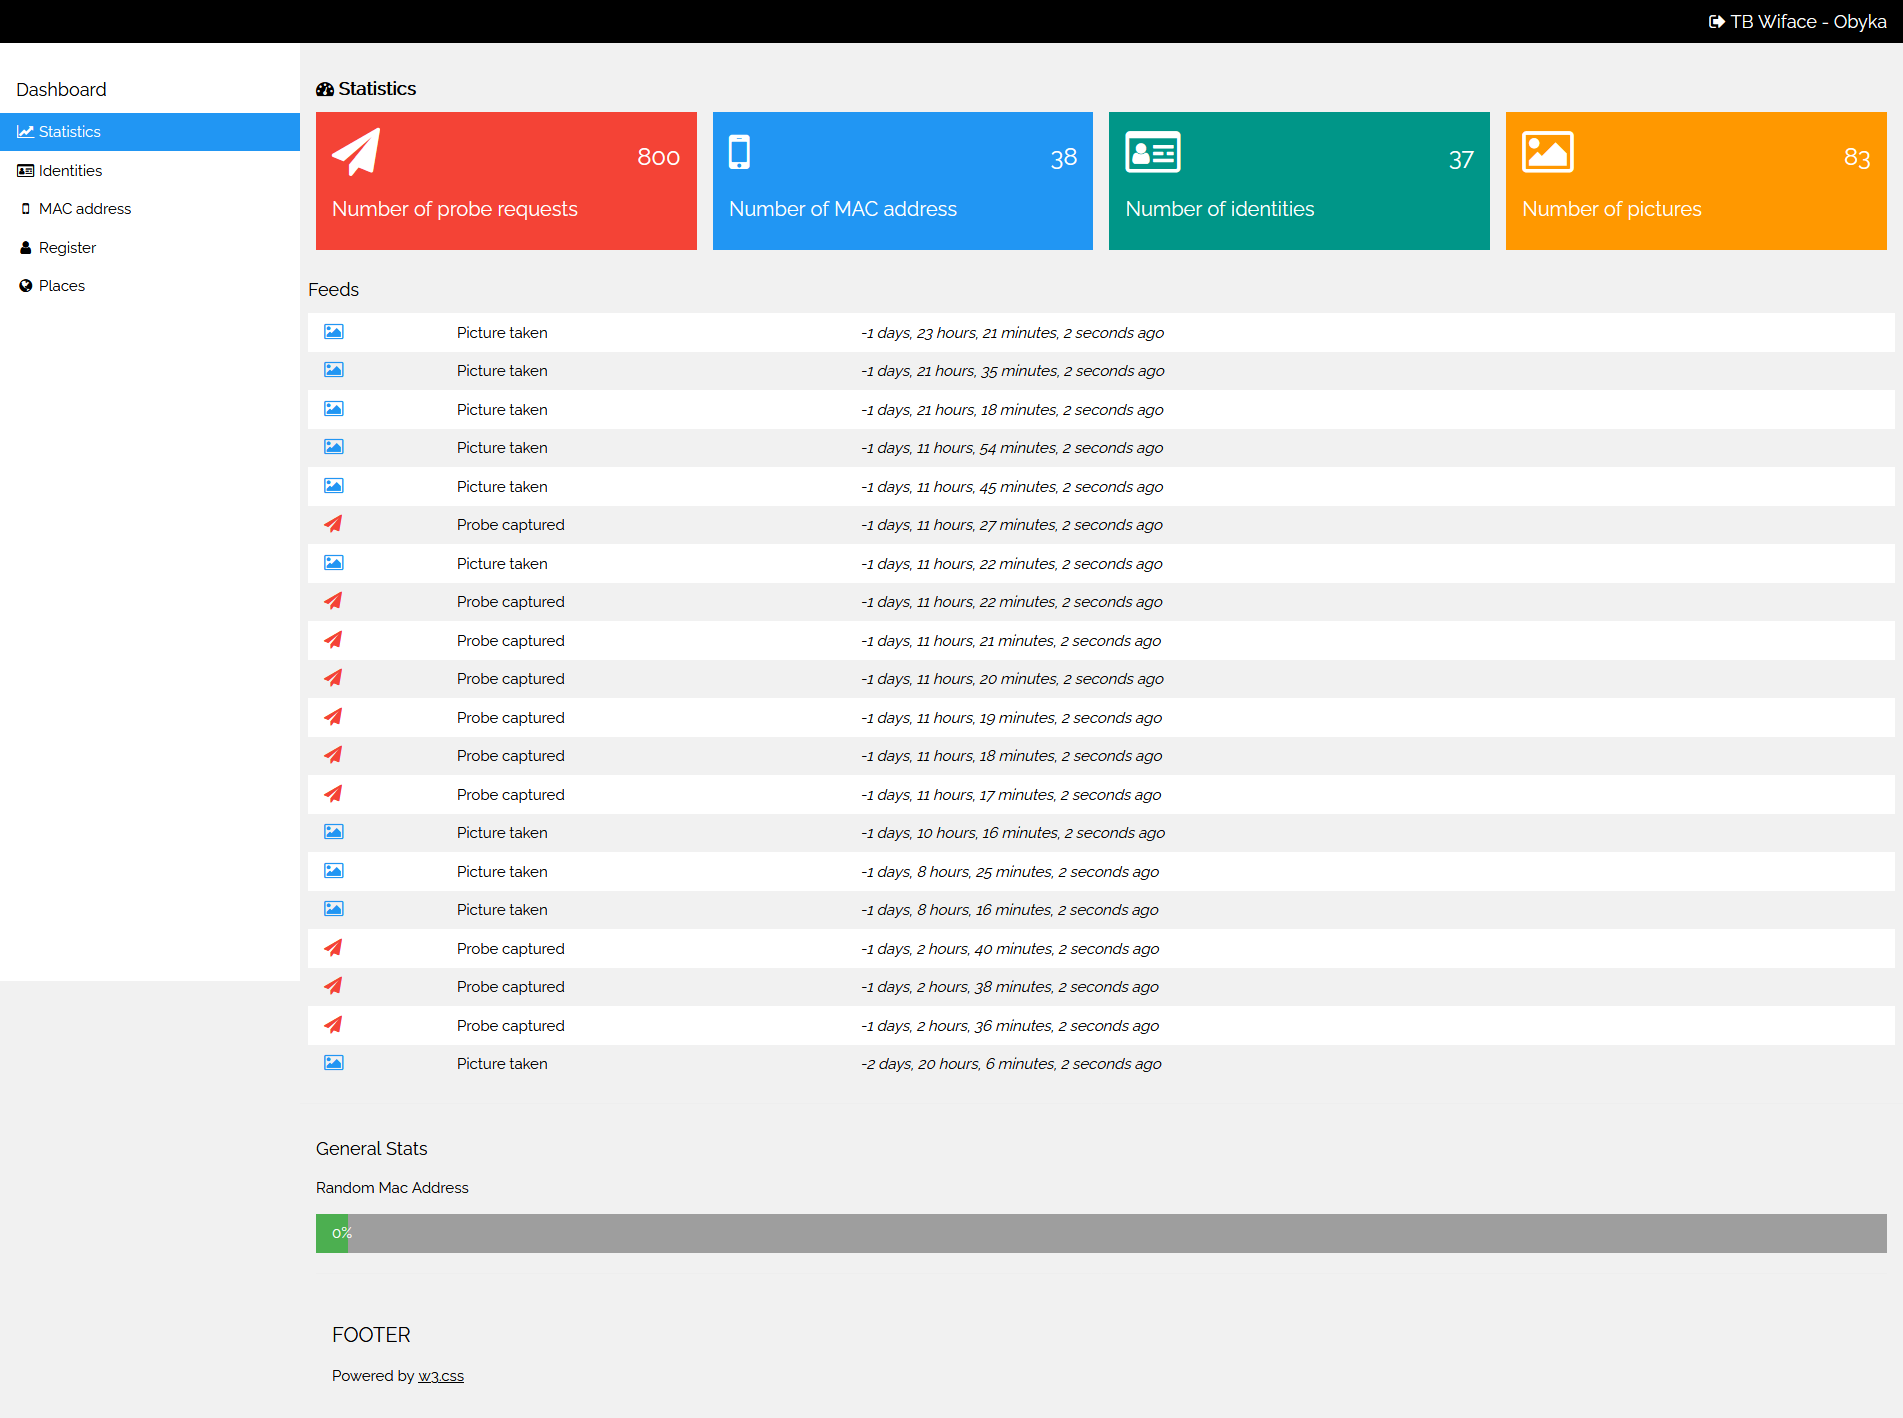
\includegraphics[width=0.95\textwidth]{images/dashboard/statistics.png}
	\caption{Page d'accueil}
	\label{fig:dashboard_stats}
\end{figure}
\end{landscape}

\subsection{Identités}
Les pages de cette section permettent de gérer les identités crées par l'API.

La page "List of Identities" (fig \ref{fig:dashboard_list_identities}) permet de naviguer parmi toutes les entrées de la base de données et affiche les données clés.
Depuis cette page, il est possible d'inclure ou non une identité dans l'algorithme PP2I. (Il pourrait par exemple être pertinent de ne pas inclure les opérateurs du système)
et aussi de supprimer une identité (ce qui supprimera aussi toutes les données hébergées par Amazon à son sujet - dans la mesure des conditions d'utilisation d'Amazon).

La page "Detailled profile" (fig \ref{fig:dashboard_identity}) donne tous les détails sur une identité. On y voit:
\begin{itemize}
    \item Une carte où sont représentés divers lieux où cette identité a été tracée (il est possible de cliquer sur les marqueurs)
    \item Les informations personnelles telles que le nom, le prénom, l'adresse e-mail
    \item Les informations engendrées par l'API telles que le nombre de photos prises de cette personne, son adresse MAC potentielle et une estimation de son âge
    \item Un avatar généré automatiquement à l'aide de features telles que les émotions, le genre, l'âge etc. permettant de visualiser une caricature de la personne sans consulter ses photographies
    \item La "meilleure" photographie de la personne (après avoir appuyé sur le bouton "Show picture")
\end{itemize}

Il est également possible d'interagir avec une identité. En appuyant sur le bouton "Updata data", l'algorithme PP2I est relancé avec l'état de la base de données actuel.
En cliquant sur le nom, prénom, ou mail de la personne, il est possible de le modifier. Une fois fait, un clic en dehors du profil envoie les nouvelles données et les actualise.

\clearpage
\newpage
\thispagestyle{empty}
\begin{landscape}
    \centering
\thispagestyle{empty}
\begin{figure}[H]
	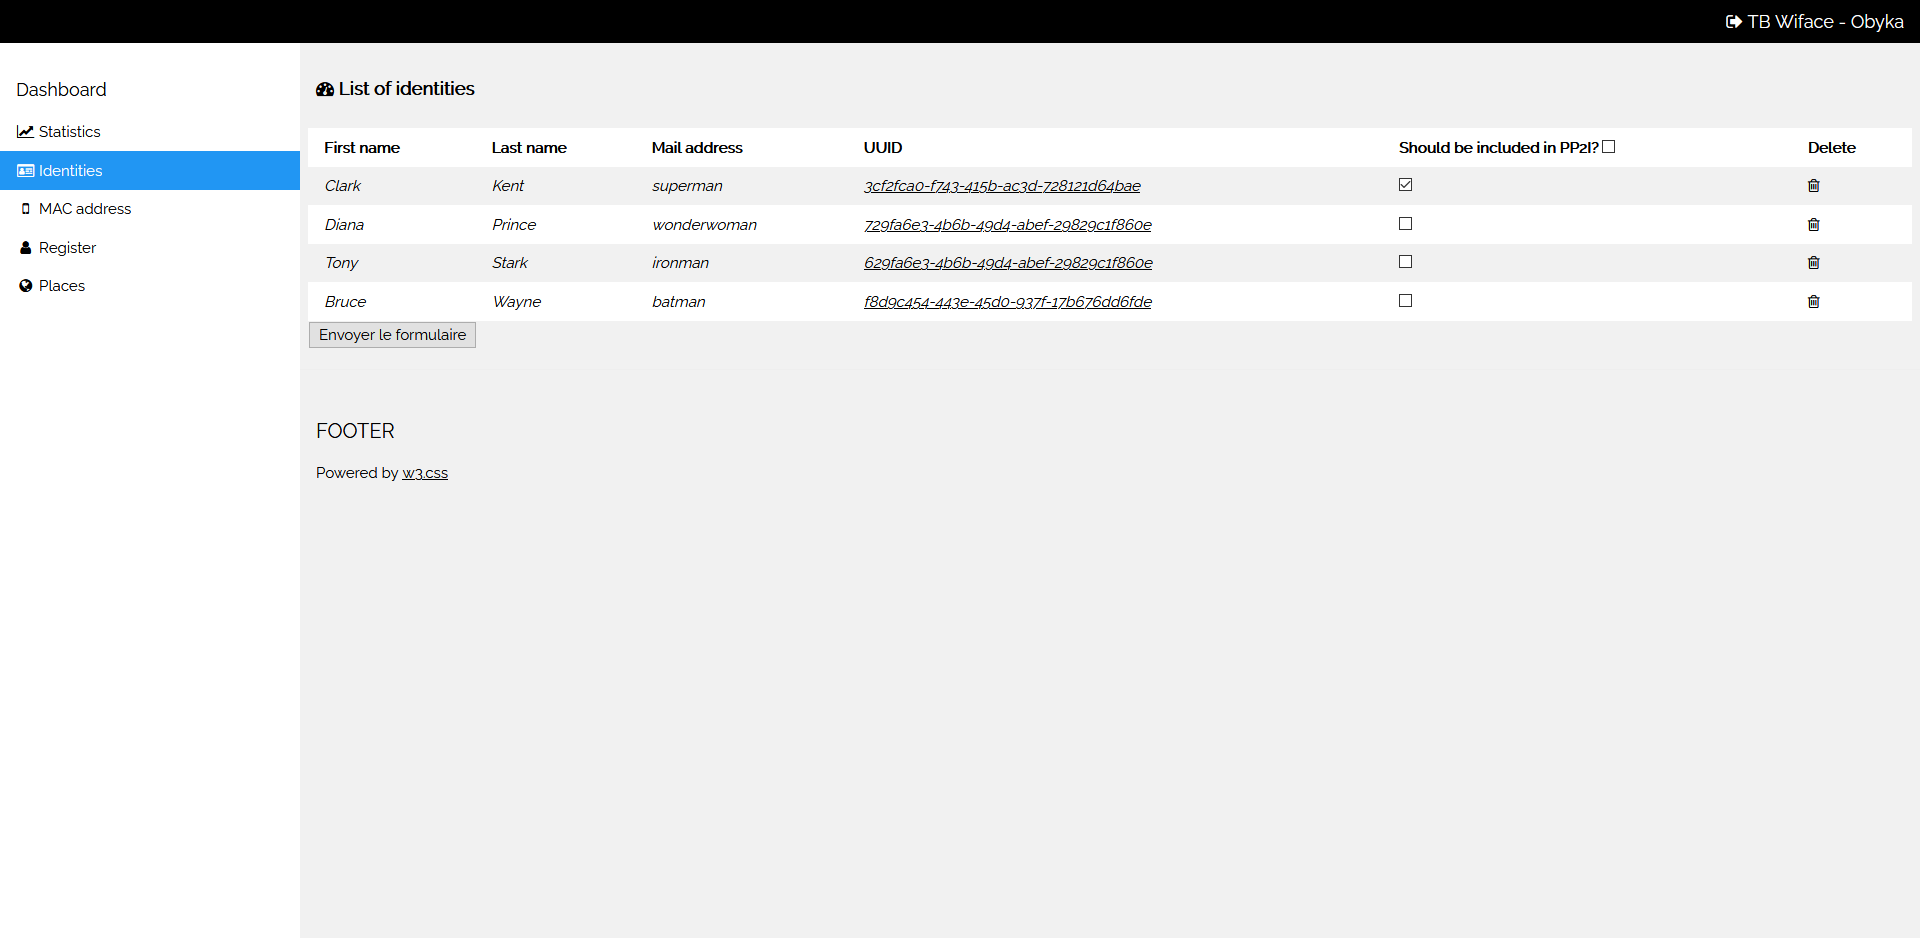
\includegraphics[width=0.95\linewidth]{images/dashboard/identities.png}
	\caption{Page listant les identités}
	\label{fig:dashboard_list_identities}
\end{figure}
\end{landscape}

\clearpage
\newpage
\thispagestyle{empty}
\begin{landscape}
    \centering
\thispagestyle{empty}
\begin{figure}[H]
	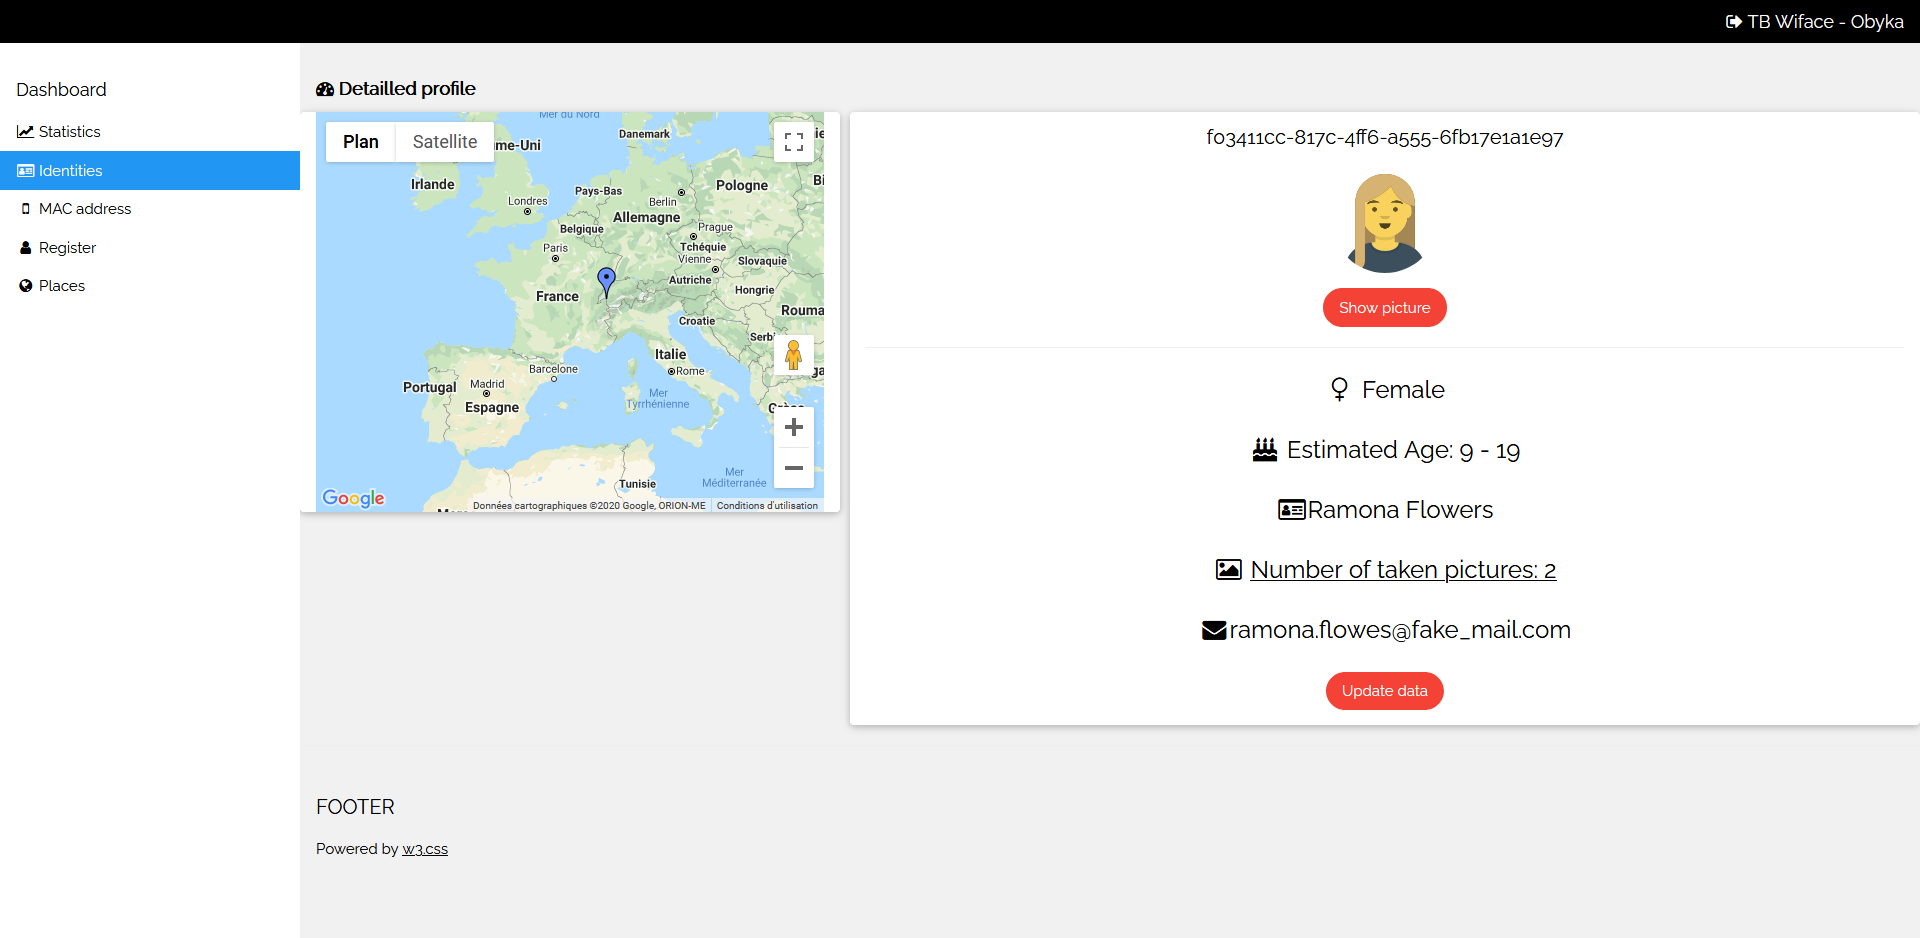
\includegraphics[width=0.95\linewidth]{images/dashboard/detailled_identities.png}
	\caption{Page détaillant une identité}
	\label{fig:dashboard_identity}
\end{figure}
\end{landscape}

\subsection{Adresses MAC}
Les pages de cette section permettent de gérer les adresses MAC présentés dans la base de données.

La page "List of MAC Addresses" (fig \ref{fig:dashboard_list_macs}) permet de naviguer parmi toutes les entrées de la base de données et affiche les données clés.
Depuis cette page, il est possible d'inclure ou non une adresse NAC dans l'algorithme PP2I. (Il pourrait par exemple être pertinent de ne pas inclure les devices appartenants aux opérateurs du système)
et aussi de supprimer une adresse.

La page "Detailled MAC address" (fig \ref{fig:dashboard_macs}) donne tous les détails sur une adresse MAC. On y voit:
\begin{itemize}
    \item une carte où sont représentés divers lieux où les probes requests provenant de cette adresse ont été capturées,
    \item l'adresse,
    \item le nombre de probe requests capturées,
    \item le constructeur potentiel de l'appareil basé sur le OUI de l'adresse \ref{ch:probe_req},
    \item le résultat des différentes heuristiques qui déterminent si une adresse est randomisée ou non.
\end{itemize}

\clearpage
\newpage
\thispagestyle{empty}
\begin{landscape}
    \centering
\thispagestyle{empty}
\begin{figure}[H]
	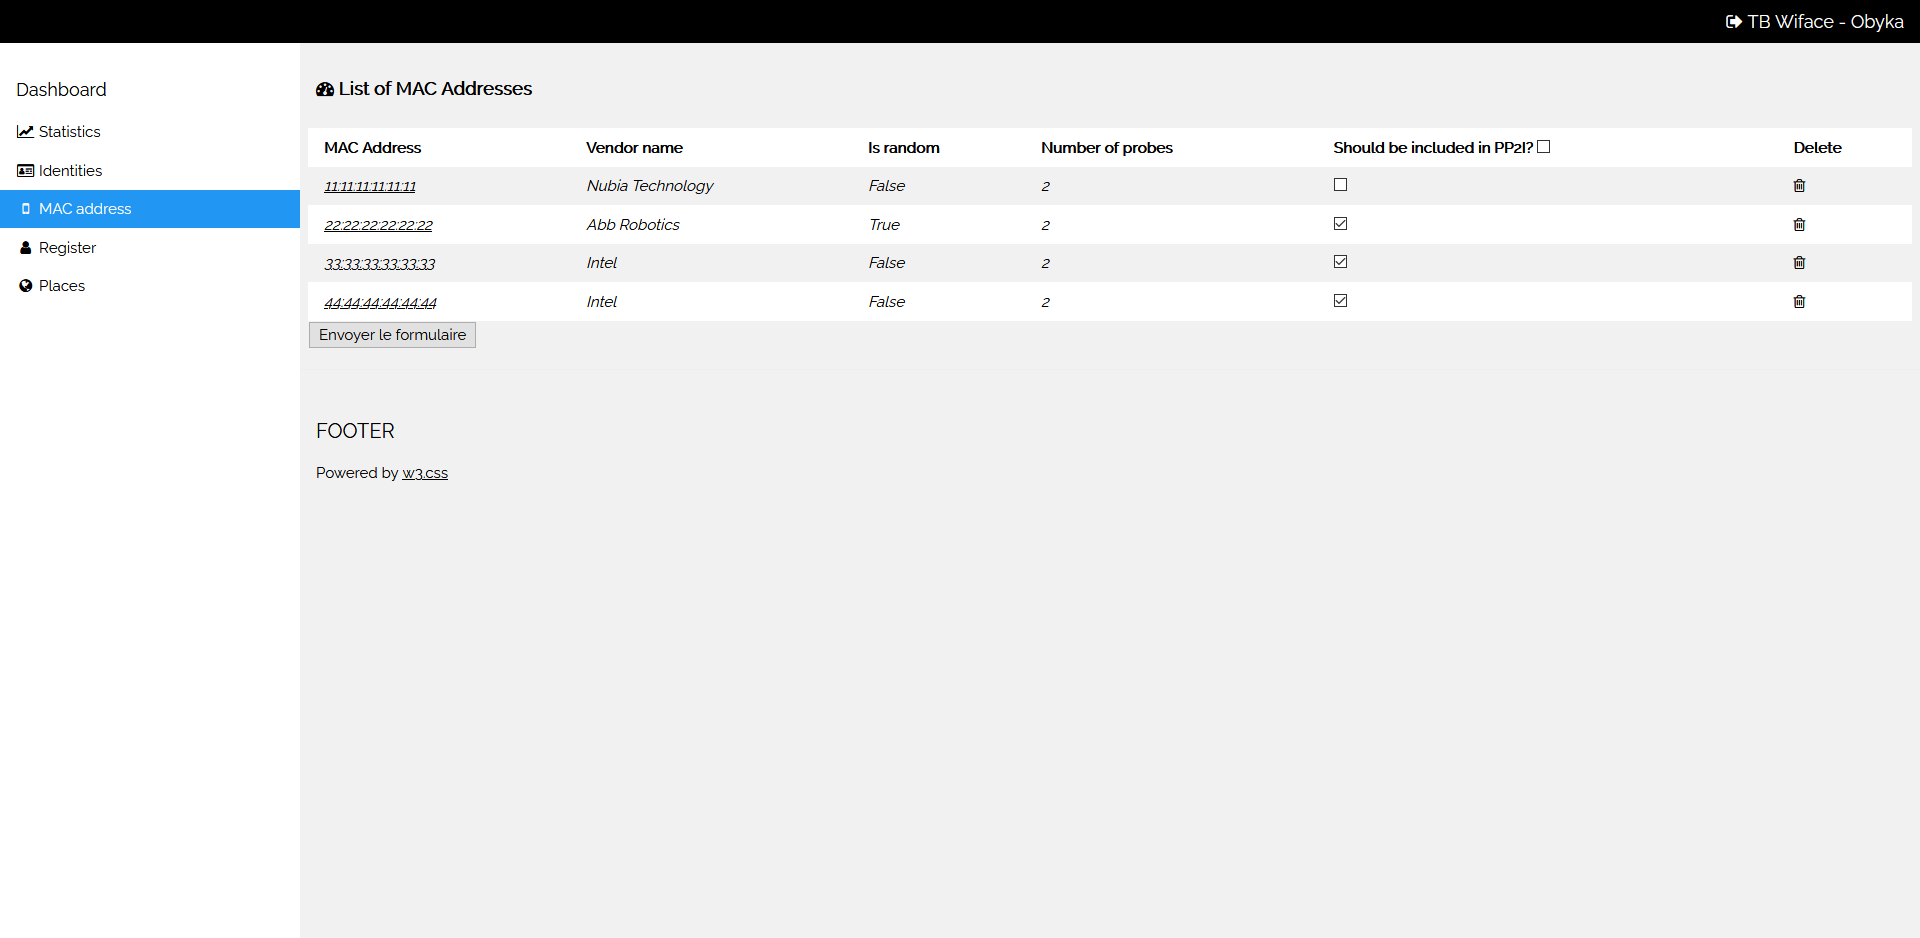
\includegraphics[width=0.95\linewidth]{images/dashboard/macs.png}
	\caption{Page listant les adresses MAC}
	\label{fig:dashboard_list_macs}
\end{figure}
\end{landscape}

\clearpage
\newpage
\thispagestyle{empty}
\begin{landscape}
    \centering
\thispagestyle{empty}
\begin{figure}[H]
	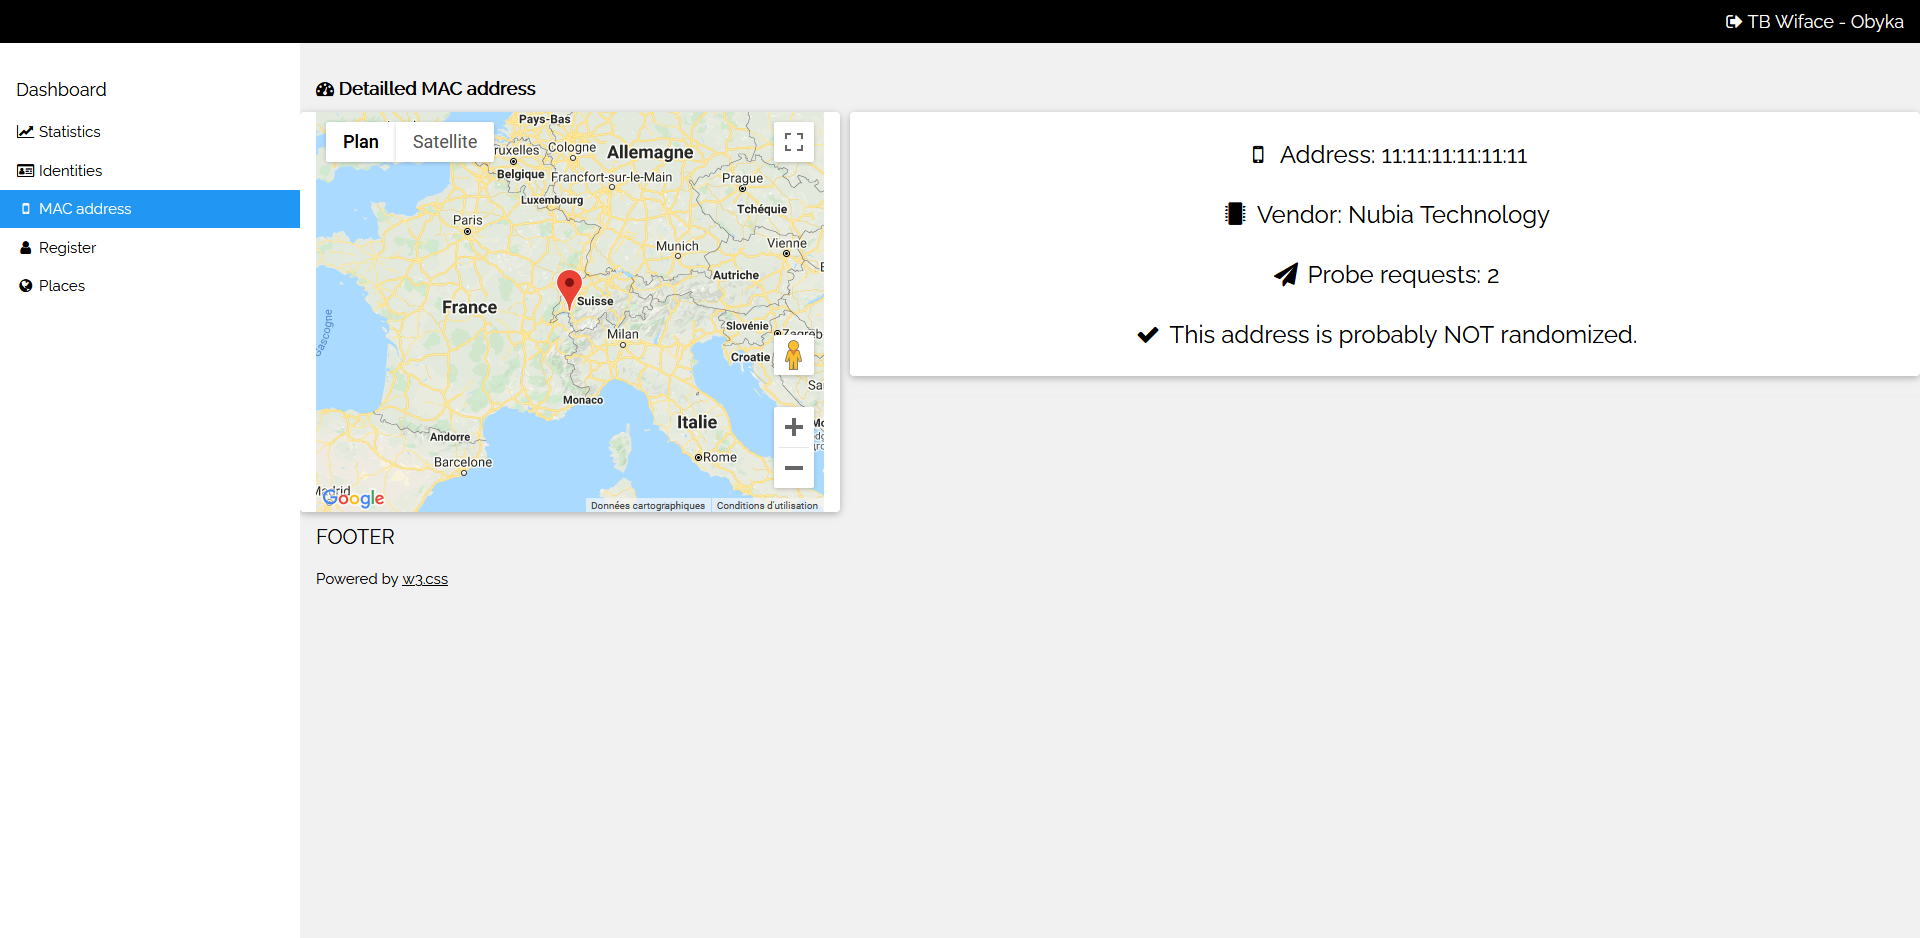
\includegraphics[width=0.95\linewidth]{images/dashboard/detailled_macs.png}
	\caption{Page détaillant une adresse MAC}
	\label{fig:dashboard_macs}
\end{figure}
\end{landscape}

\subsection{Photographies}
Les pages de cette section permettent de visualiser les images présentes dans la base de données.

La page "List of pictures" (fig \ref{fig:dashboard_list_pictures}) montre les images associées à une identité particulière et 
permet d'accèder aux images détaillées en cliquant sur ces dernières.

La page "Detailled picture" (fig \ref{fig:dashboard_picture}) donne tous les détails sur une image. On y voit:
\begin{itemize}
    \item L'avatar correspondant à l'image
    \item L'image en appuyant sur le bouton "Show Picture"
    \item Les émotions que semblent exprimer le sujet de la photo (données provenant de Rekognition)
\end{itemize}

\clearpage
\newpage
\thispagestyle{empty}
\begin{landscape}
    \centering
\thispagestyle{empty}
\begin{figure}[H]
	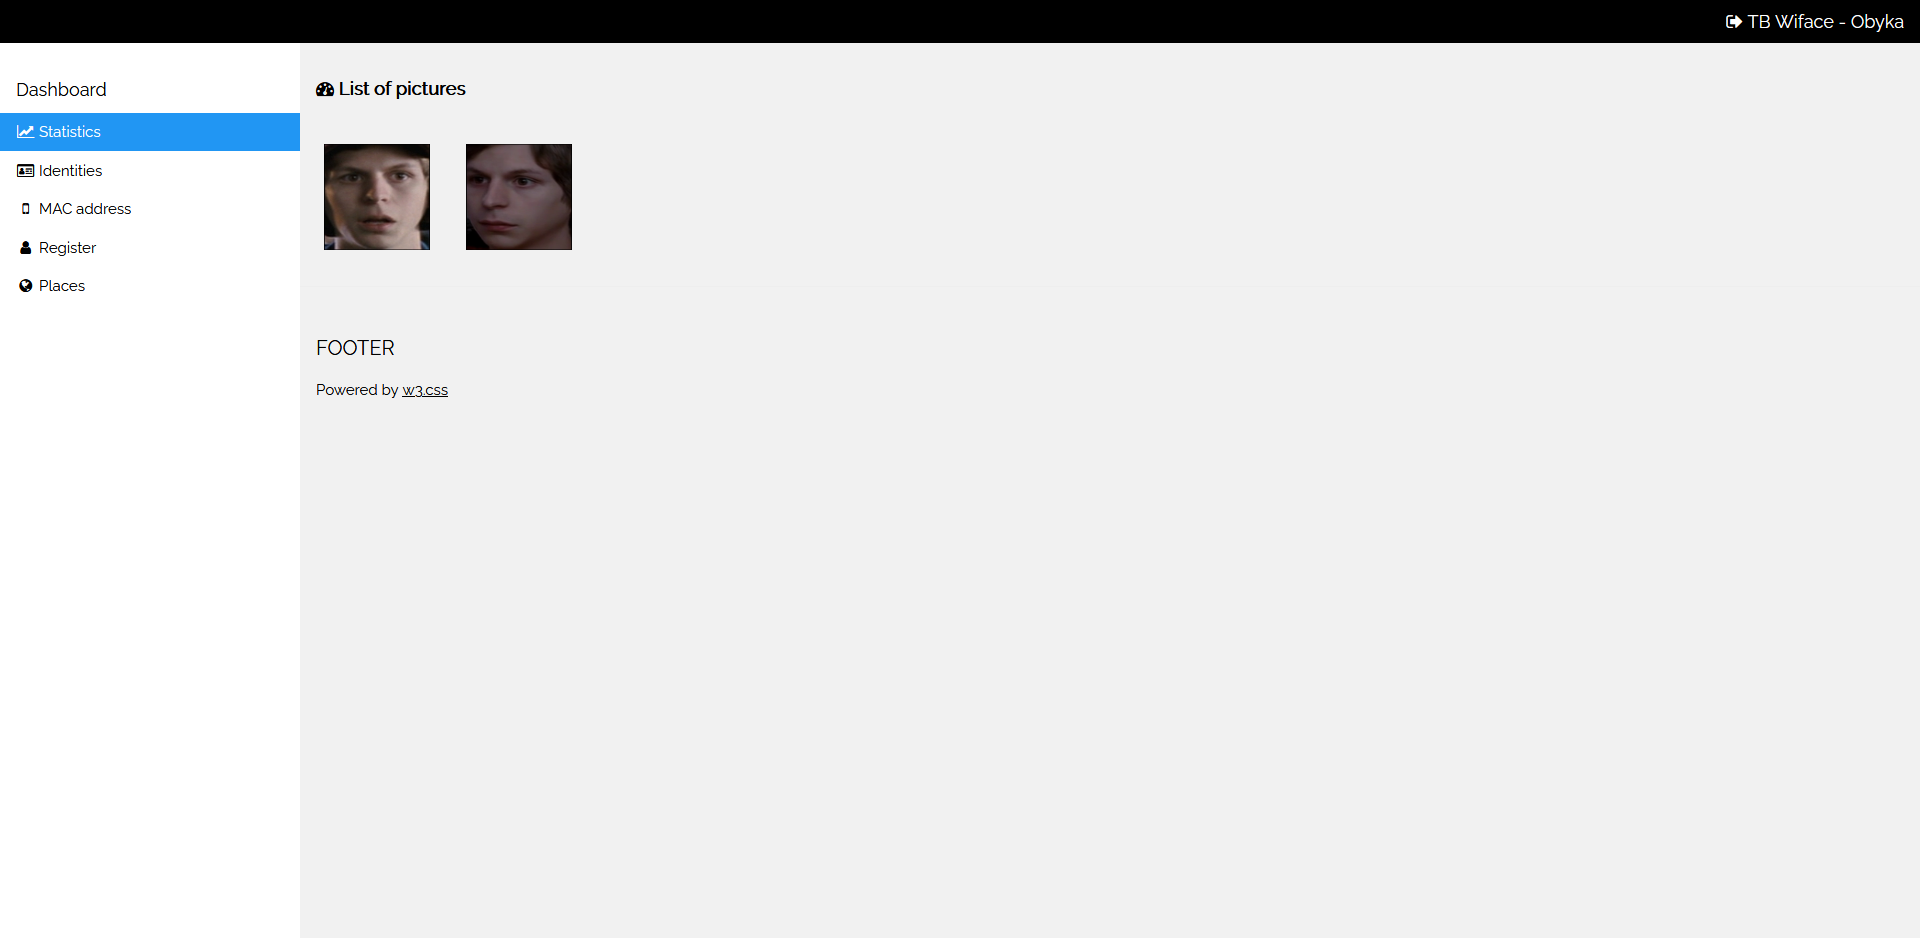
\includegraphics[width=0.95\linewidth]{images/dashboard/pictures.png}
	\caption{Page listant les adresses images associées à une identité}
	\label{fig:dashboard_list_pictures}
\end{figure}
\end{landscape}

\clearpage
\newpage
\thispagestyle{empty}
\begin{landscape}
    \centering
\thispagestyle{empty}
\begin{figure}[H]
	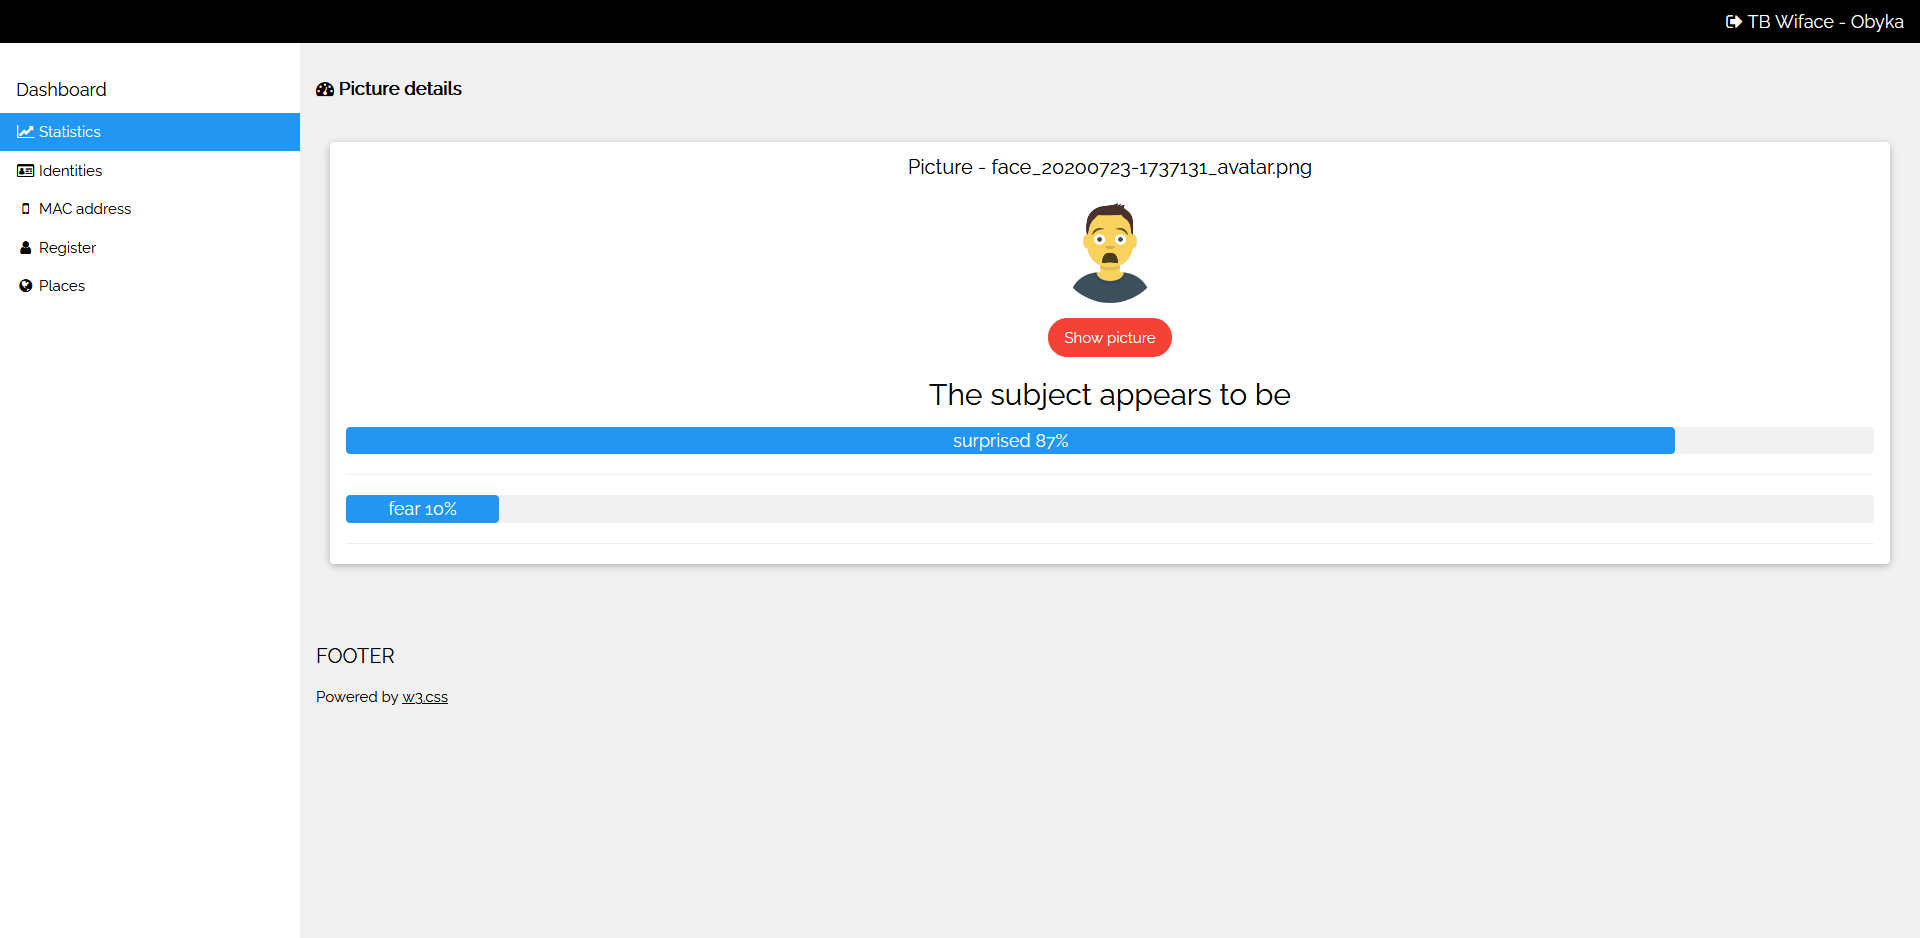
\includegraphics[width=0.95\linewidth]{images/dashboard/detailled_pictures.png}
	\caption{Page détaillant une image}
	\label{fig:dashboard_picture}
\end{figure}
\end{landscape}

\subsection{Lieux}
Les pages de cette section permettent de visualiser les lieux présentés dans la base de données.

La page "List of places" (fig \ref{fig:dashboard_list_places}) liste les différents lieux existant et permet d'accèder aux détails d'un lieu en particulier.

La page "Detailled place" (fig \ref{fig:dashboard_place}) donne tous les détails sur un lieu. On y voit:
\begin{itemize}
    \item Sa position géographique sur une carte et son nom
    \item L'âge moyen des visiteurs
    \item La proportion homme/femme de visiteurs
    \item Le nombre de visiteurs reconnus
    \item Le nombre de probe requests capturées
    \item Les émotions qui semblent être principalement ressenties par les individus se trouvant à cet endroit
\end{itemize}

La majorité de ces données peuvent être utiles à des fins marketing.

\clearpage
\newpage
\thispagestyle{empty}
\begin{landscape}
    \centering
\thispagestyle{empty}
\begin{figure}[H]
	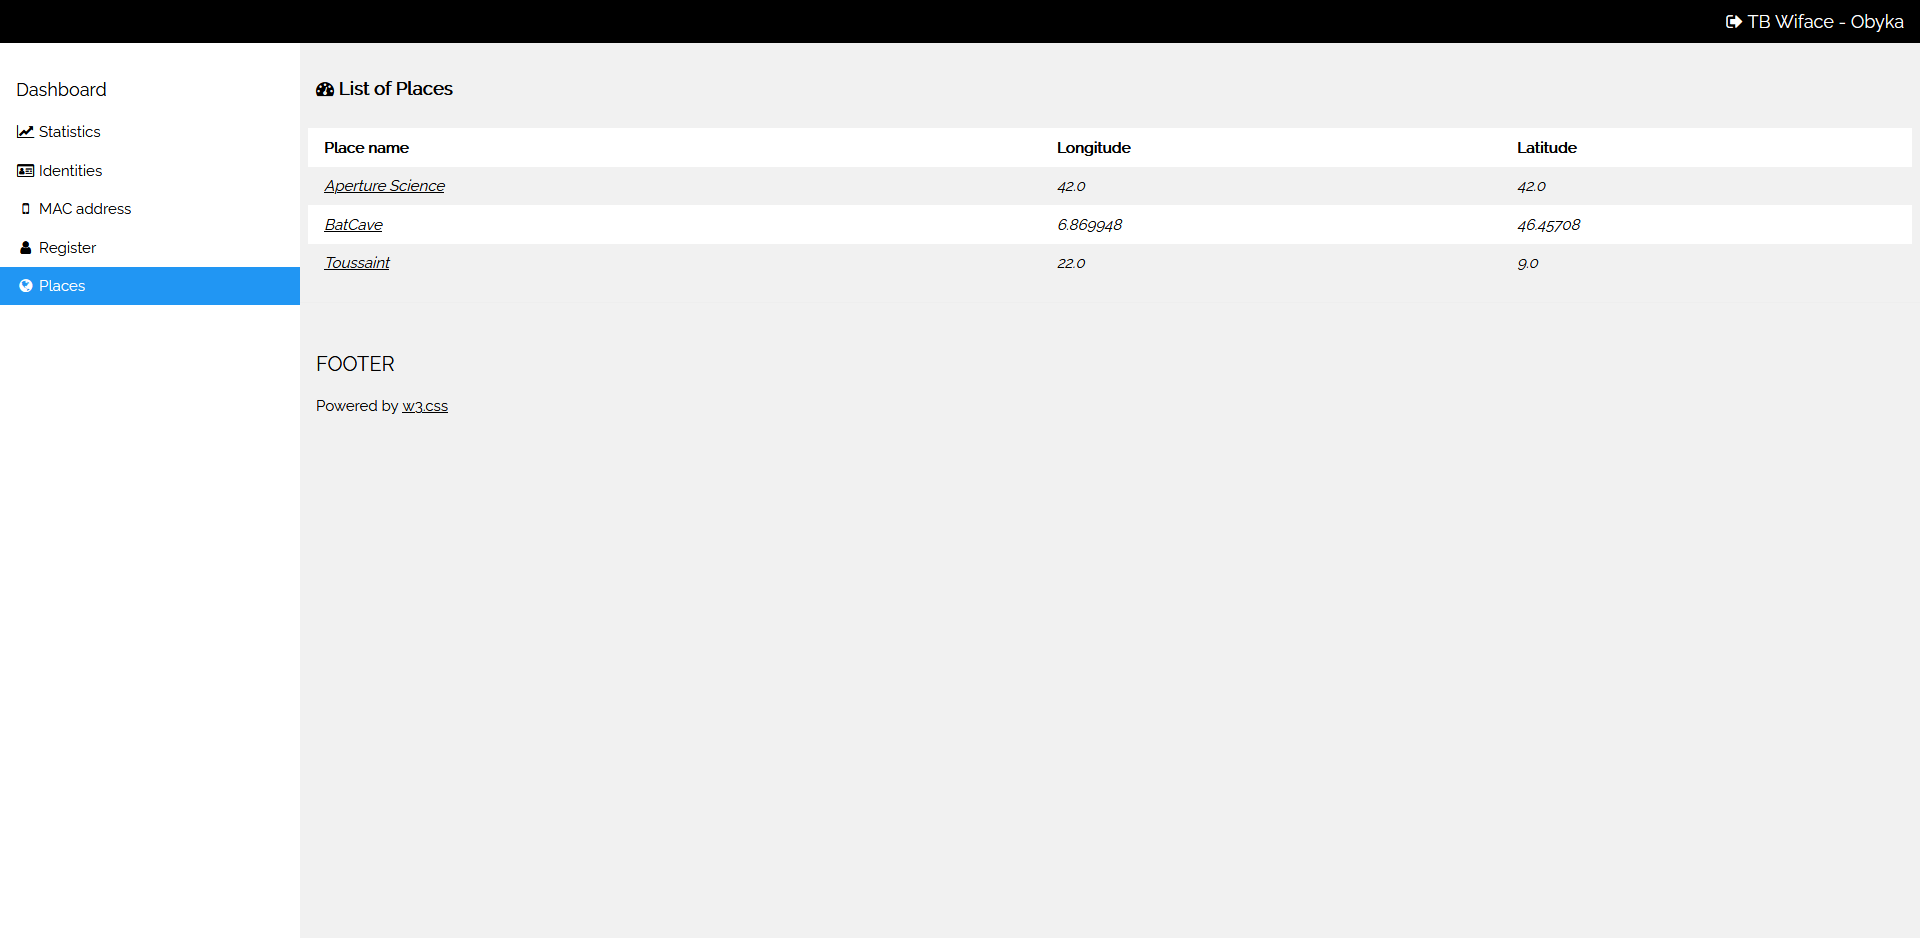
\includegraphics[width=0.95\linewidth]{images/dashboard/places.png}
	\caption{Page listant les lieux présents dans la base de données}
	\label{fig:dashboard_list_places}
\end{figure}
\end{landscape}

\clearpage
\newpage
\thispagestyle{empty}
\begin{landscape}
    \centering
\thispagestyle{empty}
\begin{figure}[H]
	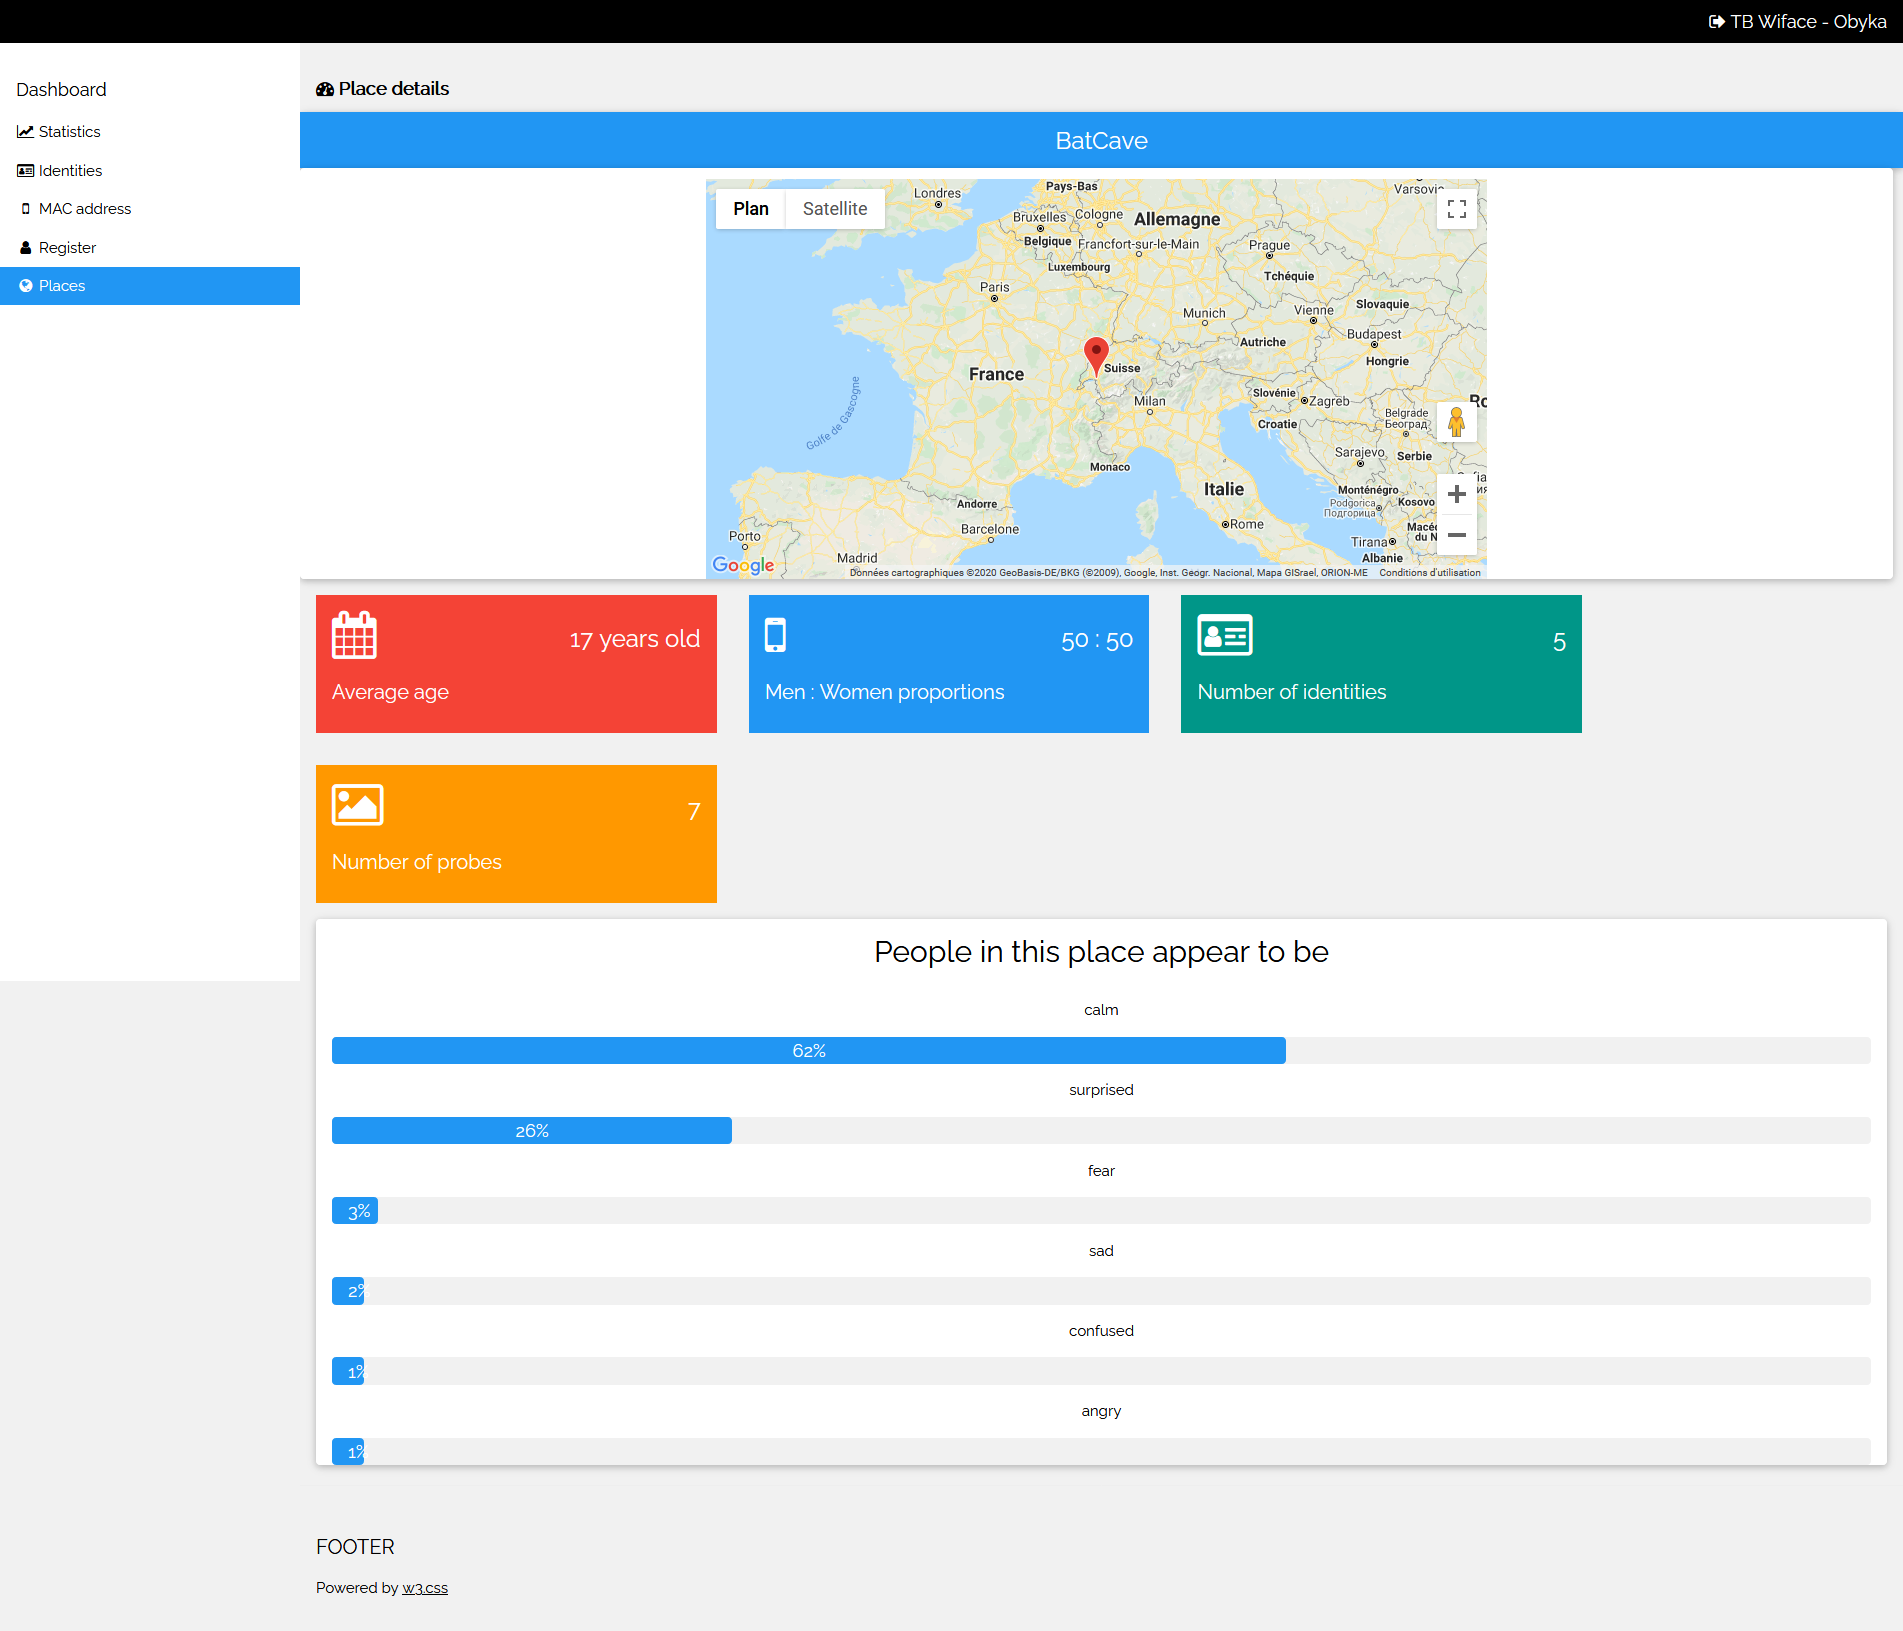
\includegraphics[width=0.84\linewidth]{images/dashboard/detailled_place.png}
	\caption{Page détaillant un lieu}
	\label{fig:dashboard_place}
\end{figure}
\end{landscape}